%!TEX TS-program = xelatex
\documentclass[]{friggeri-cv}
\usepackage{afterpage}
\usepackage{hyperref}
\usepackage{color}
\usepackage{xcolor}
%encoding
%--------------------------------------
\usepackage[T1]{fontenc}
\usepackage[utf8]{inputenc}
%--------------------------------------
 
%Portuguese-specific commands
%--------------------------------------
\usepackage[brazil]{babel}
%--------------------------------------
 
%Hyphenation rules
%--------------------------------------
\usepackage{hyphenat}
\hyphenation{mate-mática recu-perar}
%--------------------------------------

\hypersetup{
    pdftitle={},
    pdfauthor={},
    pdfsubject={},
    pdfkeywords={},
    colorlinks=false,       % no lik border color
   allbordercolors=white    % white border color for all
}
\addbibresource{bibliography.bib}
\RequirePackage{xcolor}
\definecolor{pblue}{HTML}{0395DE}

\begin{document}
\header{Kássia}{Catarine}
      {Desenvolvedora Full Stack}
      
% Fake text to add separator      
\fcolorbox{white}{gray}{\parbox{\dimexpr\textwidth-2\fboxsep-2\fboxrule}{%
.....}}

% In the aside, each new line forces a line break
\begin{aside}
  \section{Endereço}
    Quadra 604 conj. 1, 18
    Recanto das Emas, Distrito Federal
    ~
  \section{Telefone}
    (43) 9 8451-3741
    ~
  \section{Email}
    \href{mailto:kassia_catarine.15@hotmail.com}{\textbf{kassia\_catarine.15@}\\hotmail.com}
    ~
  \section{Git}
    \href{https://github.com/kassiacatarine}{kassiacatarine}
    ~
    \section{Linkedin}
    \href{https://www.linkedin.com/in/kassialopes/}{kassialopes}
    ~
  \section{Conhecimentos}
    % 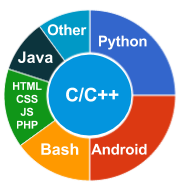
\includegraphics[scale=0.62]{img/programming.png}
    \item Git e GitHub
    \item HTML/CSS
    \item Javascript/Typescript
    \item C/C\#/Java
    \item Angular
    \item DotNet Core
    \item NodeJs/Express
    \item React
    \item Docker
    \item MySql/PostgreSQL
    \item SQL Server
    \item Mongodb
    \item Testes Unitários
    \item CI/CD
    \item Azure/Azure DevOps
    \item Scrum/Kanban
    ~
  \section{OS Preference}
    \textbf{GNU/Linux}
\includegraphics[scale=0.40]{img/5stars.png}
    \textbf{Windows}
\includegraphics[scale=0.40]{img/4stars.png}
    \textbf{Unix}
\includegraphics[scale=0.40]{img/4stars.png}
    \textbf{MacOS}
\includegraphics[scale=0.40]{img/4stars.png}
    ~
%   \section{Personal Skills}
%     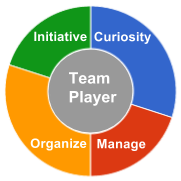
\includegraphics[scale=0.62]{img/personal.png}
%     ~
\end{aside}

\section{Experiência}
\begin{entrylist}
    \entry
    {05/20 - Agora}
    {Desenvolvedora Full Stack}
    {Luby}
    {Atividade: Criação e manutenção de telas e fluxos do backend de acordo com protótipos, para apoiar sistemas financeiros e de eventos, atuando com metodologias de desenvolvimento ágeis (Kanban e Scrum).\\\\
    Principais Tecnologias: HTML5, CSS3, Javascript, C\#, ASP.NET MVC, SQL Server.}
    \entry
    {08/19 - 01/20}
    {Estágio de Desenvolvedora Full Stack}
    {Forlogic}
    {Atividade: Implantação e manutenção de serviços em nuvem na plataforma do Azure, trabalhando com Web Apps, banco de dados Sql Azure e integração de CI/CD de aplicativos.\\
    Prototipação de novos serviços, levantamento de requisitos e desenvolvimento de aplicações web.\\\\
    Principais Tecnologias: Azure, Azure DevOps, HTML5, CSS3, Javascript, Typescript, Angular, C\#, ASP.NET Core, ASP.NET MVC, Extjs, SQL Server, Stimulsoft.}
    \entry
    {03/19 - 12/19}
    {Monitora de Programação Orientada a Objetos}
    {UTFPR - CP}
    {Atividade: Auxiliar alunos que possuíam dificuldades relacionadas ao conceito de orientação a objetos e a utilização de linguagens de programação no desenvolvimento de aplicação de console, desktop, web e mobile.\\\\
    Principais Tecnologias: Java, HTML5, CSS3.}
    \entry
    {08/18 - 04/19}
    {Desenvolvedora Full Stack}
    {Forlogic}
    {Atividade: Desenvolver sites para apoiar escolas e assistentes sociais na distribuição de bolsas escolares de colégios adventistas, realizando tarefas de levantamento de requisitos, criando protótipos, desenvolvendo e realizando manutenção.
    \\\\
    Principais Tecnologias: Azure DevOps, HTML5, CSS3, Javascript, Typescript, Angular, C\#, ASP.NET Core, ASP.NET MVC, SQL Server, Stimulsoft.}
    \entry
    {01/18 - 07/18}
    {Estágio Desenvolvedora Full Stack}
    {Forlogic}
    {Atividade: Desenvolver plataformas web para apoiar as atividades realizadas pela comunidade Adventista, atuando com metodologias de desenvolvimento ágeis (Kanban e Scrum).\\\\
    Principais Tecnologias: VSTS (Azure DevOps), HTML5, CSS3, Typescript, Angular, C\#, ASP.NET Core, SQL Server, Stimulsoft.}
\end{entrylist}

\newpage

\section{Educação}
\begin{entrylist}
  \entry
    {2015 - 2020 \\(Cursando)}
    {Bacharelado em Engenharia de Software}
    {Universidade Tecnológica Federal do Paraná, Campus Cornélio Procópio}
    {Principais assuntos: Produção, Gerenciamento, Teste e Manutenção de Softwares, Segurança e Auditoria em sistemas, Inteligência Artificial, Realidade Virtual e Programação Distribuída.\\\\
    \emph{Título da Tese: "Implementação de uma ferramenta para anotação de variação no número de cópia usando múltiplos métodos de detecção de ponto de mudança". (Foco em Bioinformática)}\\}
%   \entry
%     {2005 - 2009}
%     {Bachelor's Degree in Computer Engineering}
%     {Università di Pisa, Italy}
%     {Main subjects: Matematics and Physics, Programming, Operational Research, Telecommunication Systems, Digital and Analogical Electronics.\\
%     \emph{Title of the Thesis: "Development, Management and Migrations of web contents and applications".}\\
%     \emph{Thesis activity carried out during an internship period at Atitlan Engineering SRL.}\\}
%   \entry
%     {2000 - 2005}
%     {Scientific Disploma.}
%     {Liceo Scientifico, Matera, Italy}
%     {Scientific Secondary School.\\
%     Main subjects: Matematics, Physics, Computer Science.}
\end{entrylist}

\section{Cursos}
\begin{entrylist}
%   \entry
%     {02/2020}
%     {NodeJs, React, React Native}
%     {Rocketseat}
%     {\emph{Semana OmniStack 10.0}}
%   \entry
%     {02/2020}
%     {React e Redux}
%     {Udemy}
%     {\emph{React, Redux e integração de APIs}}
%   \entry
%     {02/2020}
%     {React}
%     {Udemy}
%     {\emph{React 16 Definitivo}}
%   \entry
%     {02/2020}
%     {Nodejs, Express e Mongodb}
%     {Udemy}
%     {\emph{Curso básico de APIs com Nodejs + Express + Mongodb}}
%   \entry
%     {02/2020}
%     {Sass}
%     {Udemy}
%     {\emph{Sass placeholders: o jeito certo}}
  \entry
    {12/2019}
    {React}
    {Rocketseat}
    {\emph{Curso React}}
  \entry
    {12/2019}
    {NodeJs}
    {Rocketseat}
    {\emph{Curso NodeJs}}
  \entry
    {12/2019}
    {Javascript ES6}
    {Rocketseat}
    {\emph{Curso JavaScript ES6}}
  \entry
    {12/2019}
    {Javascript}
    {Rocketseat}
    {\emph{Curso JavaScript}}
  \entry
    {11/2019}
    {Web Application Security}
    {Conviso}
    {\emph{Treinamento de Web Application Security}}
  \entry
    {10/2019}
    {Jekyll}
    {Udemy}
    {\emph{Criando sites estáticos com Jekyll}}
  \entry
    {03/2019}
    {Docker}
    {Alura}
    {\emph{Docker: Criando containers sem dor de cabeça}}
  \entry
    {02/2019}
    {ASP.NET Core}
    {Alura}
    {\emph{APIs Rest com Asp.NET Core 2.1 Parte 1: Da app MVC para API}}
  \entry
    {02/2018}
    {Angular}
    {loiane.training}
    {\emph{Angular (v2+) do básico ao avançado}}
 \entry
    {07/2017}
    {Git e GitHub}
    {Udemy}
    {\emph{Git e GitHub Completo: O Guia passo a passo}}
 \entry
    {07/2017}
    {Git e Github}
    {Udemy}
    {\emph{Git e Github para iniciantes}}
 \entry
    {07/2017}
    {Java}
    {Udemy}
    {\emph{Lógica de Programação e Algoritmos em Java - Introdução}}
  \entry
    {07/2017}
    {GNU/Linux}
    {Udemy}
    {\emph{Introdução a GNU/Linux}}
  \entry
    {07/2017}
    {Typescript}
    {Udemy}
    {\emph{Iniciando com Typescript}}
\end{entrylist}

% \newpage

% \begin{aside}
% ~
% ~
% ~
%   \section{Places Lived}
%     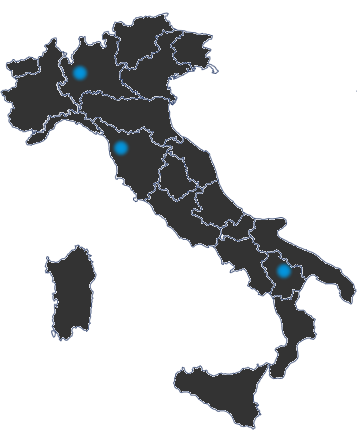
\includegraphics[scale=0.25]{img/italia.png}
%     ~
%   \section{Languages}
%     \textbf{Italian}
\includegraphics[scale=0.40]{img/5stars.png}
%     \textbf{English}
\includegraphics[scale=0.40]{img/4stars.png}
% \end{aside}

% \section{Publications}
% C. Benedetto, E. Mingozzi, C. Vallati\\
% \textbf{A Handoff Algorithm based on Link Quality Prediction for Mass Transit Wireless Mesh Networks}\\
% \emph{Proceedings of the 18th IEEE Symposium on Computers and Communications (ISCC 2013), Split, Croatia, July 7-10, 2013}
% \\
% \section{Outras Informações}
% For the Italian job market:\\
% \emph{Si autorizza il trattamento delle informazioni contenute nel curriculum in conformità alle disposizioni previste dal d.lgs. 196/2003. Si dichiara altresì di essere consapevole che, in caso di dichiarazioni non veritiere, si è passibili di sanzioni penali ai sensi del DPR 445/00 oltre alla revoca dei benefici eventualmente percepiti.}
% \\
% \begin{flushleft}
% \emph{January 14th, 2014}
% \end{flushleft}
% \begin{flushright}
% \emph{Carmine Benedetto}
% \end{flushright}

%% This piece of code has been commented by Karol Kozioł due to biblatex errors. 

% \printbibsection{article}{article in peer-reviewed journal}
% \begin{refsection}
%  \nocite{*}
%  \printbibliography[sorting=chronological, type=inproceedings, title={international peer-reviewed conferences/proceedings}, notkeyword={france}, heading=subbibliography]
% \end{refsection}
% \begin{refsection}
%  \nocite{*}
%  \printbibliography[sorting=chronological, type=inproceedings, title={local peer-reviewed conferences/proceedings}, keyword={france}, heading=subbibliography]
% \end{refsection}
% \printbibsection{misc}{other publications}
% \printbibsection{report}{research reports}

\end{document}
